\chapter*{3 Versuchsdurchführung und Auswertung}
\addcontentsline{toc}{chapter}{3 Versuchsdurchführung und Auswertung}
\setcounter{chapter}{3}
\setcounter{section}{0}
\setcounter{subsection}{0}

        \begin{table}[H]
            \centering
            \caption{Messwerte Versuch 1}
            \vspace*{1em}
            \begin{tabular}{|l|l|l|l|}
                \hline
                & Abstand $a_{n}$ & Abstand $L$ & Gitterkonstante $g_{n}$\\
                \hline
                $n = 1$ & $19,0\ \mathrm{cm}$ & $150,0\ \mathrm{cm}$ & $9,99\ \mathrm{\mu m}$\\
                \hline
                $n = 2$ & $38,3\ \mathrm{cm}$ & $150,0\ \mathrm{cm}$ & $9,91\ \mathrm{\mu m}$\\
                \hline
            \end{tabular}
        \end{table}
 
        \section{Versuch 1, Oberflächenspannung von Wasser und Ethanol mit der Abreißmethode}
        \label{sec:Versuch1}

        \subsection{Aufbau}

        \begin{figure}[H]
            \centering
            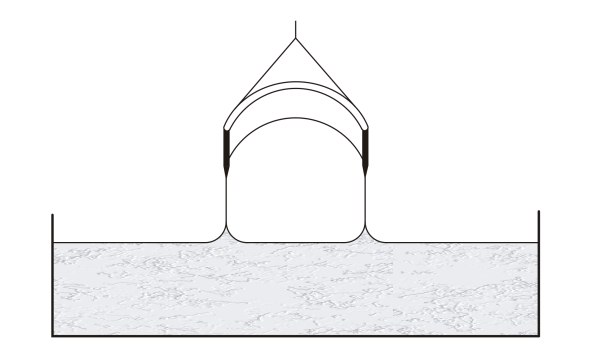
\includegraphics[width=0.8\textwidth]{bilder/Versuch1_Aufbau.png}
            \caption{Versuchsaufbau Versuch 1 \ref{an:Anleitung}}
            \label{fig:Versuch1_Aufbau}
        \end{figure}

        Um die Oberflächenspannung einer Flüssigkeit mit der Abreißmethode zu bestimmen,
        braucht man einen Metallring, einen Federkraftmesser und eine mit einer Flüssigkeit gefüllten Schale. Nun taucht man den Ring in die Flüssigkeit und misst die maximale Kraft $\mathrm{F}$, die nötig ist um den Ring wieder herauszuziehen. Die Oberflächenspannung $\sigma$ lässt sich dann mit folgender Formel bestimmen:

        \begin{equation}
            \sigma = \frac{\mathrm{F}}{2\pi d}
            \label{eq:Oberflächenspannung}
        \end{equation}
        Wobei $\mathrm{d}$ hier dem Durchmesser des Rings entspricht. Dieser beträgt TODO.
        
        Nun befestigt man einen Federkraftmesser mit dem Ring an einem Stativ und bringt dieses senkrecht über der Flüssigkeit an. TODO Genauigkeit vom Federkraftmesser und Fehler von Durchmesser. 

        \noindent Nun heben wir die Flüssigkeit soweit an bis der Ring eintaucht. Diese lassen wir nun so langsam wieder herunter bis der Ring wieder herausgezogen wird. Dabei messen wir die maximale Kraft $\mathrm{F}$, die nötig ist um den Ring wieder herauszuziehen. Die abgelesene maximale Kraft beträgt $\mathrm{F}$ können wir dann in \ref{eq:Oberflächenspannung} einsetzen. Mit dieser Variante bestimmen wir $\sigma$ von demineralisiertem Wasser und Ethanol.
        \subsection{Auswertung}
        \subsection{Diskussion}

        \section{Versuch 2, Oberflächenspannung von Tensidlösungen mit der Abreißmethode}

        \subsection{Aufbau}
        Der Aufbau ist wieder gleich zu Versuch 1 und findet sich in Abb. \ref{fig:Versuch1_Aufbau}. 

        \subsection{Auswertung}
        \subsection{Diskussion}

        \section{Versuch 3, Oberflächenspannung von Wasser und SDS-Lösung mit der Kapillarmethode}

       \subsection{Aufbau}

       \begin{figure}[H]
           \centering
           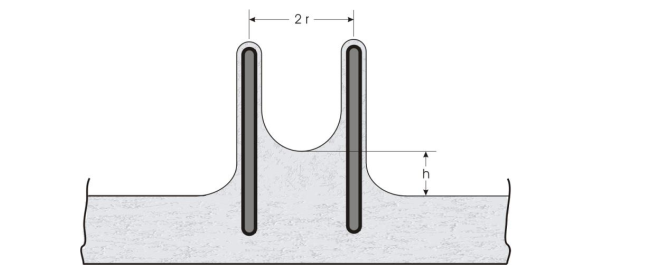
\includegraphics[width=0.8\textwidth]{bilder/Kapillarmethode.png}
           \caption{Versuchsaufbau Versuch 3 \ref{an:Anleitung}}
           \label{fig:Versuch3_Aufbau}
         \end{figure}
       \subsection{Auswertung}
         \subsection{Diskussion}

         \section{Versuch 4, Benetzung von Oberflächen}

         \subsection{Aufbau}
            \subsection{Auswertung}
            \subsection{Diskussion}
